\documentclass[12pt]{article}

\usepackage{amssymb}
\usepackage{booktabs}
\usepackage{floatrow}
\usepackage{graphicx}
\usepackage{listings}
\usepackage{url}

\title{Project}
\date{2015-10-06}
\author{Eric Scott Freeman}

\begin{document}
	\pagenumbering{gobble}
	\maketitle
	\newpage
	\tableofcontents
	\newpage
	\pagenumbering{arabic}
	\section{Introduction}
		The University of Stavanger uses an application called Autograder, written by Heine Furubotten, to automatically grade students' programming assignments. Autograder works with Github. Whenever a student pushes their code to Github, Autograder will pull a copy of the code and run a series of tests on it. Autograder does not currently have support for plagiarism detection. The goal of this project is to integrate a few anti-plagiarism tools into Autograder, thereby helping the professors save time.
		
	\section{Related Work}
		Unfortunately software plagiarism is a problem both in the classroom and in the workplace. A number of applications have been created to help detect this problem. While these tools can detect similarities in programs, the flagged files must still be manually examined to determine whether or not code was plagiarized.
		
		There are several different general techniques that are used to look for plagiarism. The tools analyzed in this project used either fingerprinting or stylometry.
	
		\subsection{Fingerprinting}
			Several tools use a technique called fingerprinting to detect plagiarism. In fingerprinting algorithms, hashes of $n$-grams, substrings that are $n$ characters, are saved and compared to help find plagiarism. Not all hashes are stored due to the large number that would be produced. 
		
			\subsubsection{Winnowing}
				Moss uses a technique called winnowing to select which hashes to save \cite{schleimer+wilkerson+aiken}. In the winnowing algorithm, a window, selection of contiguous hashes, is used to help select which hashes to save. The smallest hash from a window is saved, and then the window moves one hash over. The smallest hash from the next window is often the smallest hash from the previous window. If so it is not saved again. Figure \ref{fig:winnowing1} shows an example of how winnowing works. The orange box represents the shifting window. The green box shows whenever a new hash is saved.
				
				\begin{figure}[h!]
					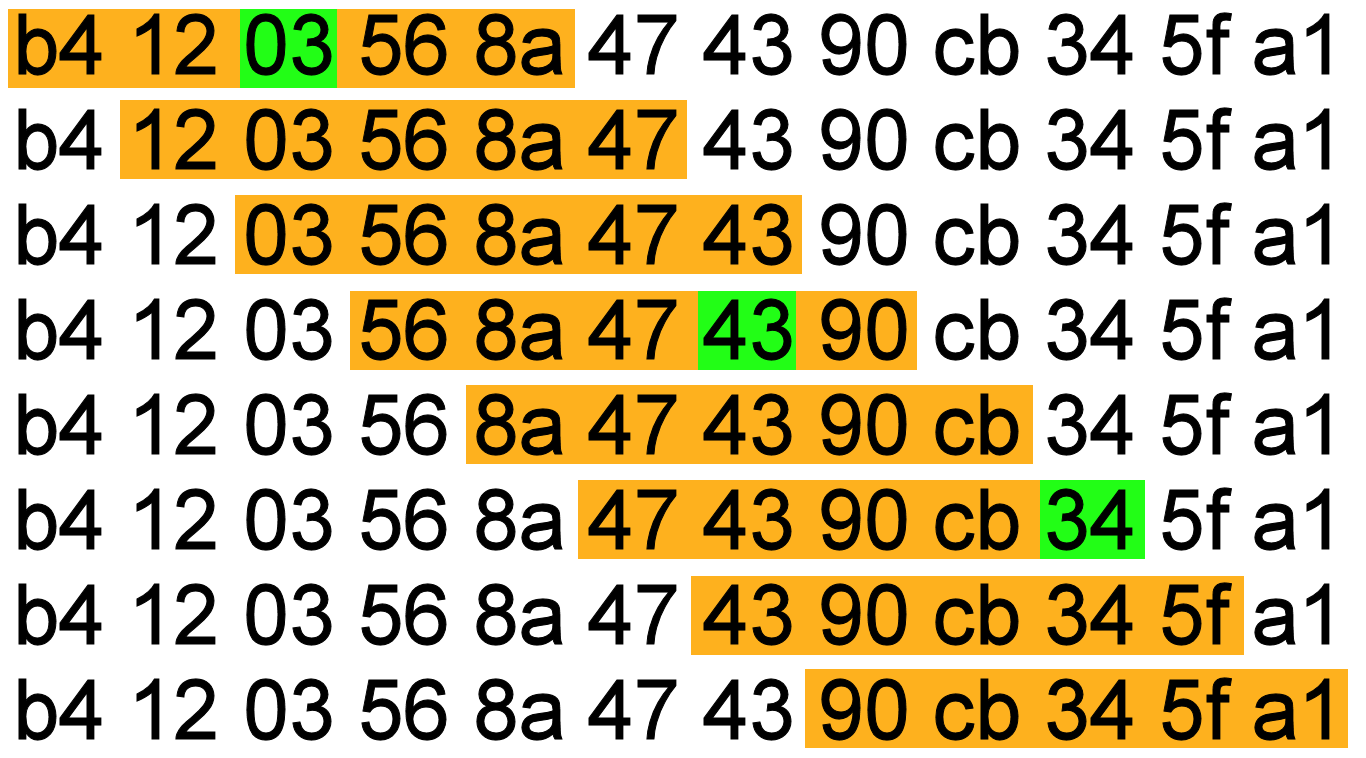
\includegraphics[scale=0.75]{Winnowing.png}
					\caption{Winnowing.}
					\label{fig:winnowing1}
				\end{figure}
			
			\subsubsection{Running-Karp-Rabin Greedy-String-Tiling}
				JPlag uses Running-Karp-Rabin Greedy-String-Tiling (RKS-GST) to compare hashes of code in plagiarism detection \cite{prechelt+malpohl+philippsen}. RKS-GST was originally used in YAP3, another plagiarism detection tool. In RKS-GST, the Greedy String half of the algorithm forms pairs of substrings, each from a different string. Then the Karp-Rabin half of the algorithm hashes each substring in the pair \cite{wise}. This is done to help detect code reordering.
		
		\subsection{Stylometry}
			Another approach is to use code stylometry, which analyzes the style of writing or coding.
			
			\subsubsection{Abstract Syntax Trees}
				Caliskan-Islam, et al. use abstract syntax trees (ASTs) to compare the styles of authors \cite{caliskan-islam+harang+liu}. Things that are easily changed in code, such as variable names, become leaves in the AST, while the structure of the tree is harder to change \cite{caliskan-islam+harang+liu}. Figure \ref{fig:ast} shows an abstract syntax tree of the code in Figure \ref{fig:astcode}. Note how the leaves, or circular nodes, in Figure \ref{fig:ast} are variable names, constants, and a function name.
				
				Michal Bohuslávek's dupl application uses ASTs to find similarities in code \cite{bohuslave}. It looks for any copies of code, not just plagiarism. So if a piece of code is duplicated even in the same file, it will test positive.
			
				\begin{figure}
					\begin{floatrow}
						\ffigbox{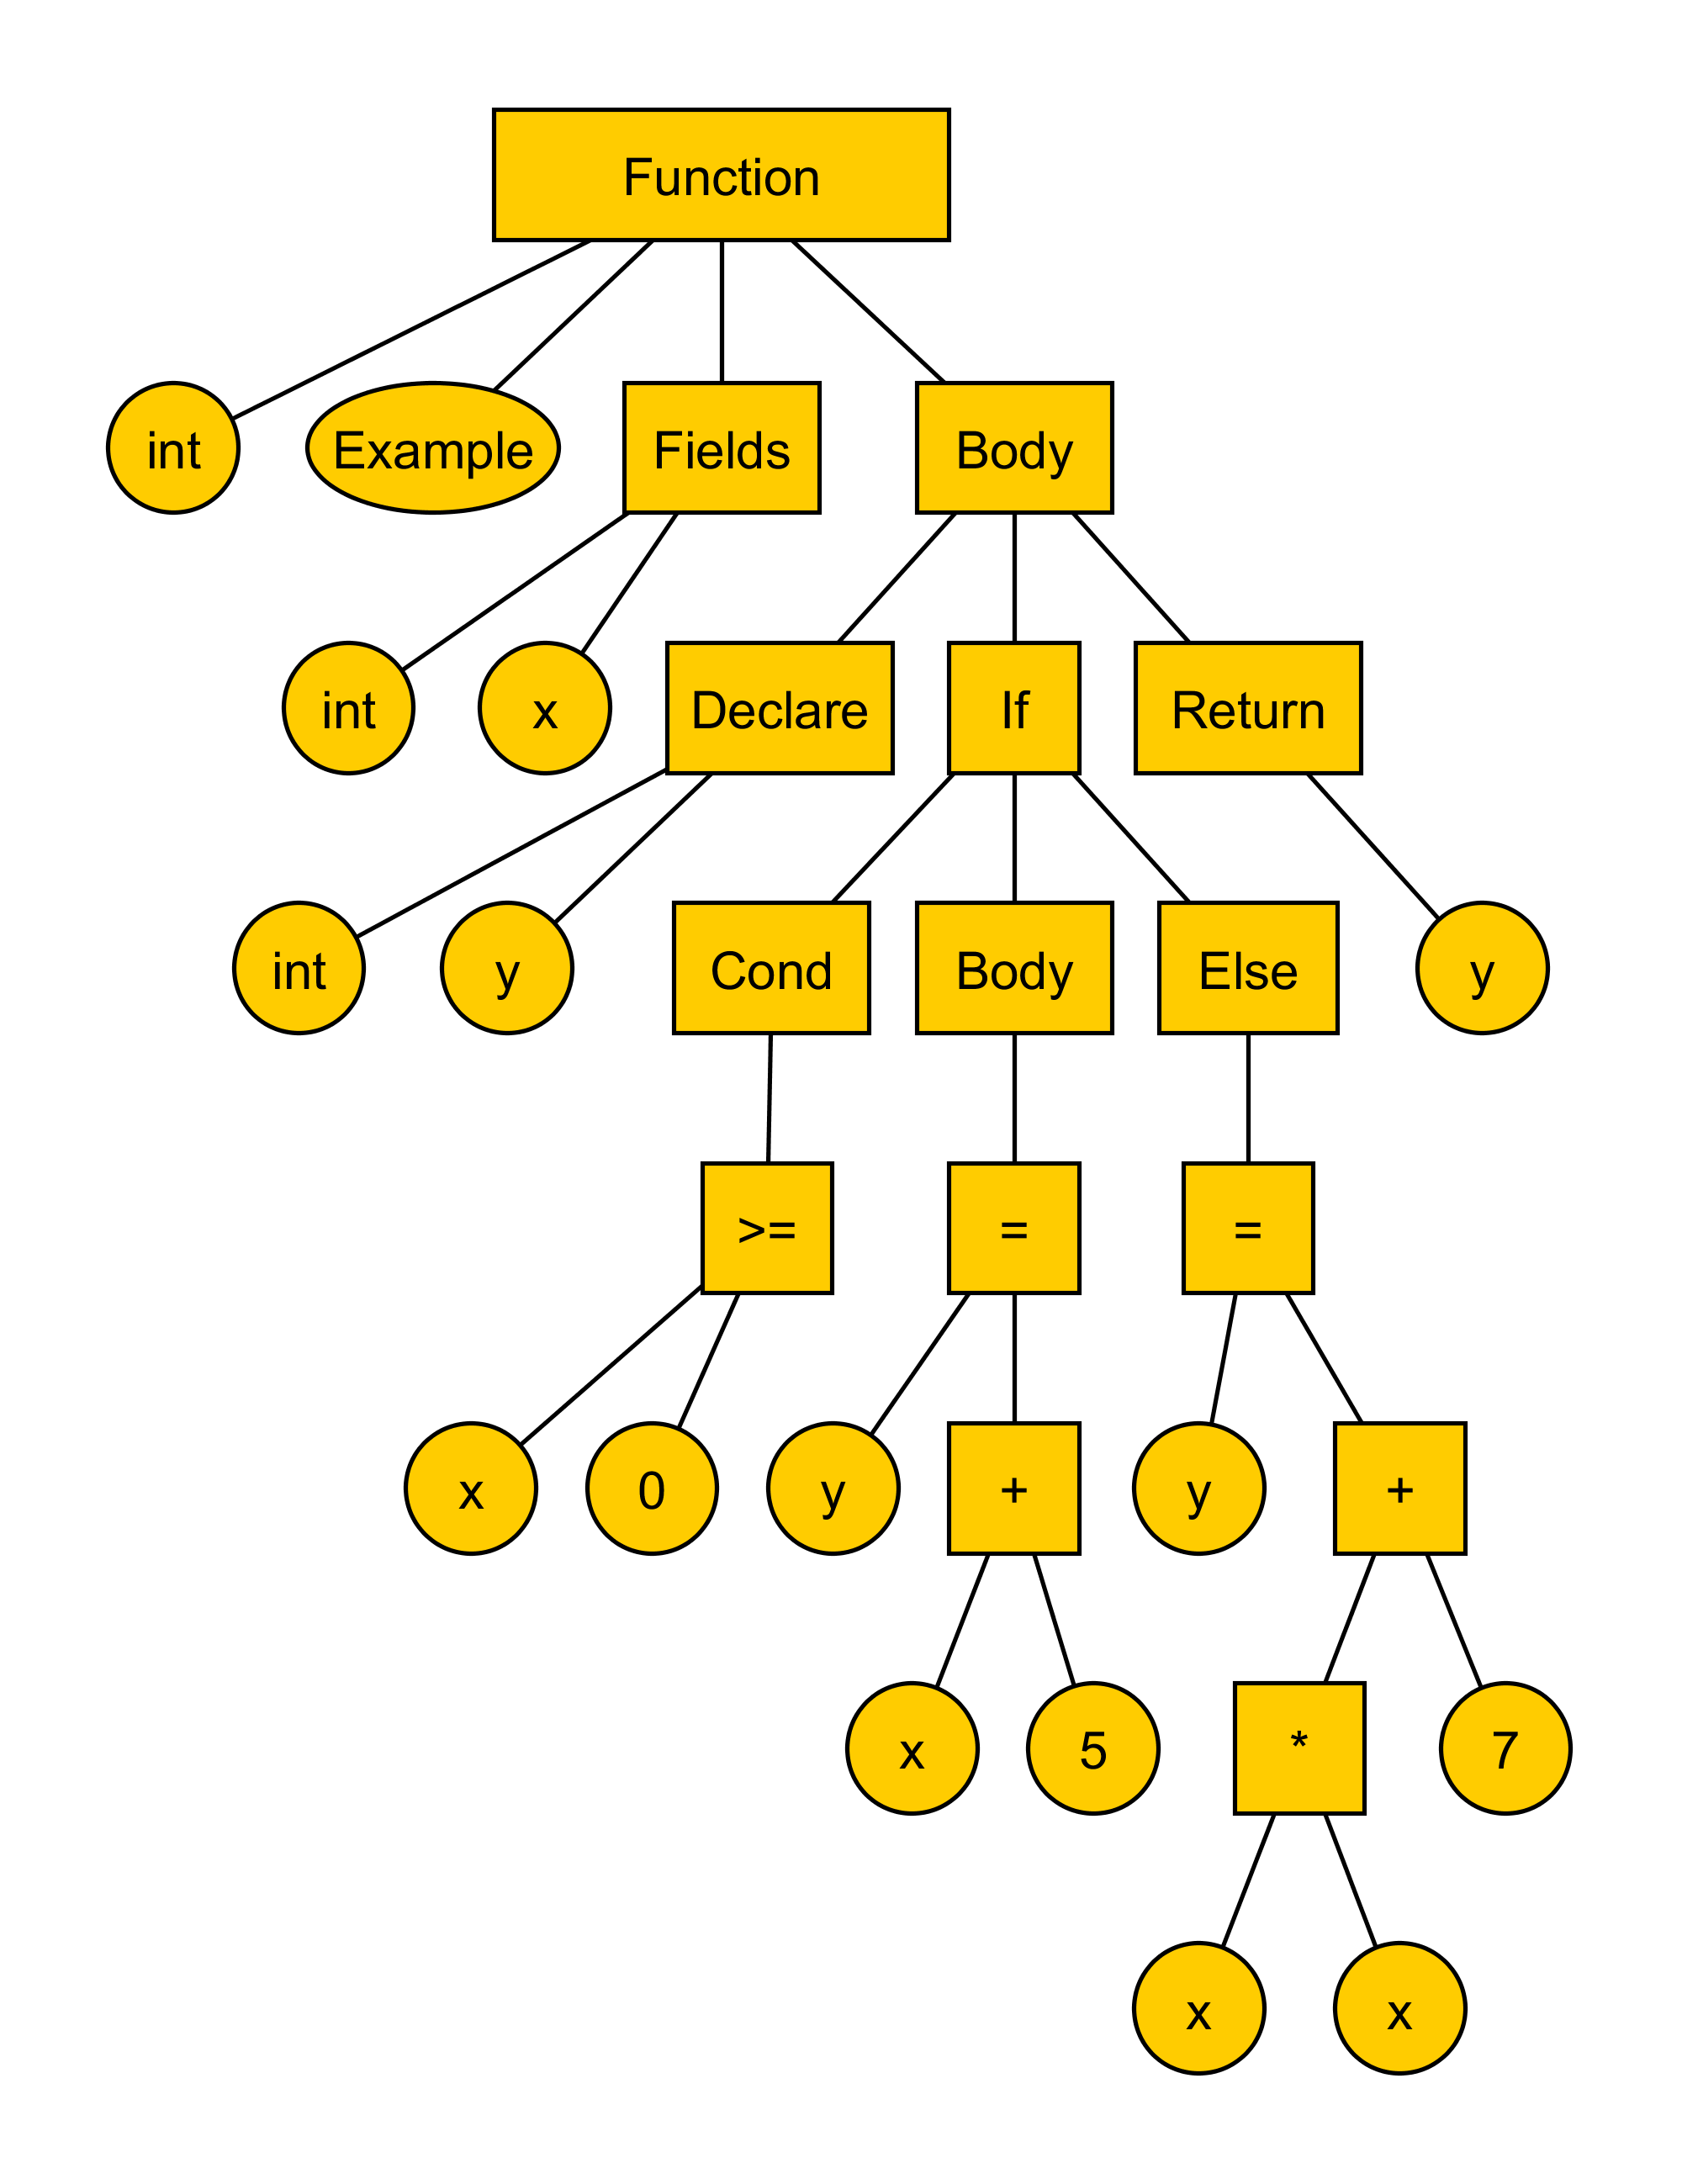
\includegraphics[scale=0.1]{AST.png}}{\caption{Abstract syntax tree.}\label{fig:ast}}	\ffigbox{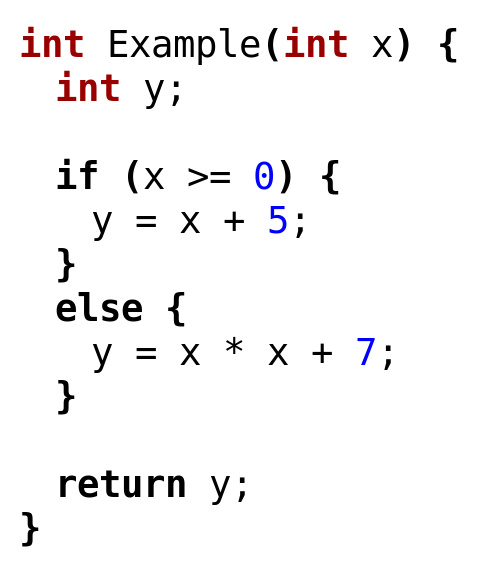
\includegraphics[scale=0.5]{ASTcode.png}}{\caption{Example code.}\label{fig:astcode}}
					\end{floatrow}
				\end{figure}
		
		\subsection{Supported Languages}
			Fingerprinting and string comparison techniques can be used to analyze source code written in languages other than their officially supported languages. Moss can analyze Go code, even though it is not technically supported. Since ASTs need to parse the code, applications which use them are stricter on which languages they can analyze. For example dupl only supports code written in Go. Table \ref{tab:languageSupport} shows the languages officially supported by several anti-plagiarism tools.
		
			\begin{table}[h!]
				\begin{center}
					\caption{Officially supported languages by various tools}
					\label{tab:languageSupport}
					\begin{tabular}{ccccccccccccccc}
						\toprule
						Tool & Java & Go & C & C\verb!++! & C\verb!#! & Python & Perl & others\\
						\midrule
						Moss & \checkmark & & \checkmark & \checkmark & \checkmark & \checkmark & \checkmark & \checkmark \\
						JPlag & \checkmark & & \checkmark & \checkmark & \checkmark & & & \checkmark\\
						Plaggie & \checkmark & & & & & & & \\
						SIM & \checkmark & & \checkmark & & & & & \checkmark\\
						dupl & & \checkmark & & & & & & \\
						\bottomrule
					\end{tabular}
				\end{center}
			\end{table}
		
	\section{Design}
		\subsection{Tools}
			Three anti-plagiarism tools were chosen for this project. Moss was the first choice because of the number of languages it supports and its maturity. JPlag and dupl were chosen to give a variety in the algorithms used.
			
			Moss is a web service, while JPlag and dupl can be run locally. To access Moss, one must send an email to \verb|moss@moss.stanford.edu| containing the following, with \verb|<email address>| replaced with one's actual email address:
			\begin{verbatim}
				registeruser
				mail <email address>
			\end{verbatim}
			\noindent Moss will then send a Moss upload script with a unique user ID, which should be placed in directory \verb|<x>|.
			
			To download and install dupl, run the following command:
			\begin{lstlisting}[language=bash]
	go get -u github.com/mibk/dupl
			\end{lstlisting}
			\noindent dupl requires Go version 1.4 or higher.
			
			To download and install JPlag, ???.
			
		\subsection{Process}
			First the students' code will be pulled from Github to the Autograder server. The directory structure will consist of a base directory containing subdirectories for each class. Inside each class, there will be directories for each student, which will have directories for each assignment. See figure \ref{fig:directories}. This is similar to how Autograder stores the files in Github, so pulling the code for the anti-plagiarism project will be simplified. Each student's work for an assignment to be compared against the other students' work for that assignment in that class. This will keep the number of files being compared from growing too large. 
			
			\begin{figure}[h!]
				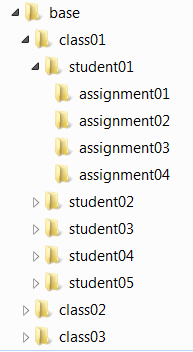
\includegraphics[scale=0.75]{Directories.png}
				\caption{Directory structure.}
				\label{fig:directories}
			\end{figure}
			
			A separate Go package will be written for each anti-plagiarism tool. The packages will implement a common interface which will create the commands to send to the tools and will format the results.
			
			Here is an example of a Moss command:
			\begin{lstlisting}[language=bash, breaklines=true]
./moss -l java -m 2 -d ./code/class01/student01/assignment01/*.java ./code/class01/student02/assignment01/*.java ./code/class01/student03/assignment01/*.java > assignment01.txt &
			\end{lstlisting}
			\noindent The first argument is the Moss upload script. The $-l$ flag signifies that the next argument will be the language the assignments were written in, which in this case is Java. The $-m$ flag signifies that the following argument will be the threshold for Moss, which tells Moss to ignore matches that appear in more than this number of files. In this example, if a piece of code appears in more than 2 files, it is ignored. This is useful if instructors provide some functions or classes for their students to use. The $-d$ option signifies that directories will be compared instead of specific files. In this example, all the java files from three students' assignment 1 will be compared. Moss will search inside subdirectories. Finally the output from Moss is sent to a text file. The text file will contain a URL that has the results from Moss.
			
			Here is an example of a dupl command:
			\begin{lstlisting}[language=bash, breaklines=true]
dupl -t 15 -html ./code/class01/student01/assignment02/ ./code/class01/student02/assignment02/ ./code/class01/student03/assignment02/ > assignment02.html &
			\end{lstlisting}
			\noindent The first argument is a call to dupl. The next argument, $-t$ is dupl's threshold. This is minimum nodes that pieces of code must be before dupl declares them as a duplicates. In this example, it is 15 nodes. $-html$ specifies html output. Next is a list of the directories. dupl will search inside subdirectories. Finally the output from dupl will be sent to an html file.
			
	\section{Results}
	\section{Analysis}
	\section{Conclusion}
	\bibliography{sources}
	\bibliographystyle{ieeetr}
\end{document}